\documentclass[twocolumn]{article}
\usepackage[utf8]{inputenc}
\usepackage{enumerate}
\usepackage{amsmath}
\usepackage{graphicx}
\usepackage{listings}
\linespread{1.05}
\usepackage[sc]{mathpazo}
\usepackage{color}
\usepackage{gensymb}
\usepackage{multicol}
\usepackage{ltxgrid}
\usepackage{float}
\usepackage{romannum}
\usepackage{times}

\title{FYS-3150 Project 2}
\author{Tobias Olesen & Thomas Sjåstad}
\date{October 4th 2017}
\begin{document}
\maketitle
\onecolumngrid
\noindent\makebox[\linewidth]{\rule{\paperwidth}{0.4pt}}
\begin{center}
\section*{Abstract} 
Our numerical approach applied to the quantum mechanical harmonic oscillator produced values related to that of analytic values. The jacobi method; used to find eigenvalues was reliable and passed tests though using some time to find them. Eigenvalues found with jacobi method was: $\lambda_1 = 2.9995$, $\lambda_2 = 6.9975$, $\lambda_3 = 10.9939$ where the analytic values are: $\lambda_1 = 3.0$, $\lambda_2 = 7.0$, $\lambda_3 = 11.0$. 

For the interacting case (two electrons in the h.o potential) the value found differed by a factor of 2 which came from the difference in scaling of equations thus giving the same answer as analytic value, $\lambda_{anl} = 0.625$. Eigenvalue for interacting case $\lambda_{num} = 1.24992 = \lambda_{anl}\cdot2$  
\end{center}  
\noindent\makebox[\linewidth]{\rule{\paperwidth}{0.4pt}}
\newline
\twocolumngrid
\section*{\Romannum{1}. INTRODUCTION}
The aim of this project is to develop a program that uses Jacobi's method for finding eigenvalues. We start with the simple case of a quantum mechanical particle moving in a potential with infinite walls, and then move on to solving Schroedinger's equation for two particles in a three-dimensional harmonic oscillator well with and without a repulsive Coloumb interaction.

We want to solve the Schroedinger equation as an eigenvalue problem.
The equation need to be reformulated in a discretized form as an eigenvalue equation to be solved with Jacobi's method.

This type of problem leads to the field of quantum dots; electrons confined in small areas in semiconductors, wich is a hot research area in modern solid-state physics.
\newline
The eigenvalue solver we want to end up with should be general enough as to possibly be applied to a range of different cases. 
An important aspect of this is to be aware of that the equations involved need to be properly scaled. This gets the equations in a simpler form, which in addition to making the equations easier to read also has other benefits: It may reduce the complexity of the problem, it makes it easier to compare (or recognize) equations with one another (possibly even from different areas of physics), it makes it easier to recognize when to apply familiar mathematical techniques, it may help avoid round-off errors and might reduce the number of times we have to solve the equation numerically.
\newline
The eigenvalue solver we want to end up with should be general enough as to possibly be applied to a range of different cases. 
An important aspect of this is to be aware of that the equations involved need to be properly scaled. This gets the equations in a simpler form, wich in addition to making the equations easier to read also has other benefits: It may reduce the complexity of the problem, it makes it easier to compare (or recognize) equations with one another (possibly even from different areas of physics), it makes it easier to recognize when to apply familiar mathematical techniques, it may help avoid round-off errors and might reduce the number of times we have to solve the equation numerically.
\newline
\section*{\Romannum{2}. METHOD/APPROACH}
\subsection*{Single electron case}
The quantum mechanical problem we want to solve is the harmonic oscillator in three dimensions where we have a central symmetric potential; that is, the potential is only dependent on the radial distance r from the origin. r goes from 0 to $\infty$. In one dimension the harmonic oscillator potential reads: $V(x) = \frac{1}{2}k x^2 $, where $k = \omega^2 m$; m is the mass of the particle and $\omega$ is the angular frequency. Changing x with r we obtain a central symmetric potential $V(r) = \frac{1}{2}kr^2$. The general Schroedinger equation is a function that is dependent on the radial distance r, two angles $\theta$ and $\phi$, which are angles rotating the radial distance vector in the room. 
\newline
The time-independent Schroedinger equation:
\begin{equation}
    \frac{-\hbar}{2m}\nabla^2\Psi + V\Psi = E\Psi
\end{equation}
$\hbar$ is a constant, m is the mass of the particle, $\nabla$ is the gradient and has the form since we are in spherical coordinates; 
\newline
$\nabla^2 = \frac{1}{r^2}\frac{\partial}{\partial r} (r^2\frac{\partial}{\partial r}) + \frac{1}{r^2\sin\theta}\frac{\partial}{\partial \theta}(\sin\theta \frac{\partial}{\partial \theta} ) + \frac{1}{r^2\sin^2\theta}(\frac{\partial^2}{\partial\phi^2 })$. 
\newline
Further we assume that $\Psi(r, \theta, \phi)$ can we separated into two functions $\Psi(r, \theta, \phi) = R(r), Y(\theta, \phi)$. $R$ is called the radial equation and $Y$ the angular equation. Substituting the two new functions R and Y into the SD(schroedinger) equation and arrange the equation to have dependency on R and Y for itself we can change the partial derivatives to ordinary derivatives and get two equations which solves for the radial part and the angular part of the wave function. With some algebra the radial equation looks like eq (2). Not all steps are shown here, complete derivation can be looked up from [1].
\newline
With the potential defined we look at the radial equation:
\begin{equation}
    -\frac{\hbar^2}{2 m} \left ( \frac{1}{r^2} \frac{d}{dr} r^2
    \frac{d}{dr} - \frac{l (l + 1)}{r^2} \right )R(r) 
    + V(r) R(r) = E R(r).
\end{equation}
l is the azimuthal quantum number that determines the orbital angular momentum and the shape of the orbital. V(r) is the potential, E is the energy which is given by $E_{nl}=  \hbar \omega \left(2n+l+\frac{3}{2}\right)$. $n = 0, 1, 2...$, $l = 0, 1, 2...$. 
\newline

We now want to get eq (2) on a simpler form and we introduce $R(r) = \frac{1}{r u(r)}$ thus collecting the separate derivatives into a double derivative:
\begin{equation}
  -\frac{\hbar^2}{2 m} \frac{d^2}{dr^2} u(r) 
       + \left ( V(r) + \frac{l (l + 1)}{r^2}\frac{\hbar^2}{2 m}
                                    \right ) u(r)  = E u(r) .
\end{equation}
For this project we are not interested in the orbital momentum and set l = 0. Wanting to simplify the equation more we introduce a dimensionless variable $\rho = \frac{r}{\alpha}$, inserting this and $V(\rho) = (1/2) k \alpha^2\rho^2$ into (3) we end up with:
\begin{equation}
  -\frac{\hbar^2}{2 m \alpha^2} \frac{d^2}{d\rho^2} u(\rho) 
       + \frac{k}{2} \alpha^2\rho^2u(\rho)  = E u(\rho) .
\end{equation}
Atlast we multiply with $2m\alpha^2/\hbar^2$ on both sides and obtain:
\begin{equation}
  -\frac{d^2}{d\rho^2} u(\rho) 
       + \frac{mk}{\hbar^2} \alpha^4\rho^2u(\rho)  = \frac{2m\alpha^2}{\hbar^2}E u(\rho) .
\end{equation}
$\alpha$ is a constant which that we decide. For easiest value we set $\frac{mk\alpha^4}{\hbar^2} = 1$ $=>$ $\alpha = (\frac{\hbar^2}{mk})^\frac{1}{4}$ cleaning up the equation and finally ending up with:    
\begin{equation*}
  -\frac{d^2}{d\rho^2} u(\rho) + \rho^2u(\rho)  = \lambda u(\rho) .
\end{equation*}
where $\lambda = \frac{2m\alpha^2}{\hbar^2}E$. 
The expression for the second derivative can be written as:
\begin{equation}
u''=\frac{u(\rho+h) -2u(\rho) +u(\rho-h)}{h^2} +O(h^2),
\end{equation}
$O(h^2)$ is the error function. h is the step size where we cut up our step size into N pieces and define a starting and ending point; $h = \frac{\rho_N - \rho_0}{N}$. In our case we will put $\rho_0 = 0$ and $\rho_{max} = 5$. This choice of $\rho_{max}$ will give us the three first eigenvalues with four leading digits. $\rho_i = \rho_0 + ih $ where i = 0, 1, 2....., N. 
Putting this in eq(6) we can write the Schroedinger equation evaluated at a point $\rho_i$ as:
\begin{equation}
-\frac{u_{i+1} -2u_i +u_{i-1} }{h^2}+\rho^2_iu_i  = \lambda u_i
\end{equation}
$V_i(\rho) = \rho^2_i$ is the harmonic potential.

We now wish to put this equation into a matrix and solving for the eigenvalues and vectors. 
We define first the diagonal matrix element
\begin{equation*}
   d_i=\frac{2}{h^2}+V_i,
\end{equation*}
and the non-diagonal matrix element
\begin{equation*}
   e_i=-\frac{1}{h^2}.
\end{equation*}
The non-diagonal matrix elements are given by a constant.
With these definitions the Schroedinger equation takes the following form
\begin{equation*}
d_iu_i+e_{i}u_{i-1}+e_{i}u_{i+1}  = \lambda u_i,
\end{equation*}
where $u_i$ is unknown and are the eigenvectors. This is the eigenvalue problem we want to solve:
\begingroup\makeatletter\def\f@size{8}\check@mathfonts
\def\maketag@@@#1{\hbox{\m@th\large\normalfont#1}}

\begin{equation*}
    \begin{bmatrix}d_0 & e_0 & 0   & 0    & \dots  &0     & 0 \\
                                e_1 & d_1 & e_1 & 0    & \dots  &0     &0 \\
                                0   & e_2 & d_2 & e_2  &0       &\dots & 0\\
                                \dots  & \dots & \dots & \dots  &\dots      &\dots & \dots\\
                                0   & \dots & \dots & \dots  &\dots  e_{N-1}     &d_{N-1} & e_{N-1}\\
                                0   & \dots & \dots & \dots  &\dots       &e_{N} & d_{N}
             \end{bmatrix}  \begin{bmatrix} u_{0} \\
                                                              u_{1} \\
                                                              \dots\\ \dots\\ \dots\\
                                                              u_{N}
             \end{bmatrix}=\lambda \begin{bmatrix} u_{0} \\
                                                              u_{1} \\
                                                              \dots\\ \dots\\ \dots\\
                                                              u_{N}
             \end{bmatrix} 
      \label{eq:sematrix}
\end{equation*}\endgroup

The boundary conditions of u are: $u(0)$ = $u(\infty)$ $= 0$ at the endpoints; we are not concerned with these values in our matrix thus getting our matrix:
\begingroup\makeatletter\def\f@size{7}\check@mathfonts
\def\maketag@@@#1{\hbox{\m@th\large\normalfont#1}}
\begin{equation*}
    \begin{bmatrix} \frac{2}{h^2}+V_1 & -\frac{1}{h^2} & 0   & 0    & \dots  &0     & 0 \\
                                -\frac{1}{h^2} & \frac{2}{h^2}+V_2 & -\frac{1}{h^2} & 0    & \dots  &0     &0 \\
                                0   & -\frac{1}{h^2} & \frac{2}{h^2}+V_3 & -\frac{1}{h^2}  &0       &\dots & 0\\
                                \dots  & \dots & \dots & \dots  &\dots      &\dots & \dots\\
                                0   & \dots & \dots & \dots  &-\frac{1}{h^2}  &\frac{2}{h^2}+V_{N-2} & -\frac{1}{h^2}\\
                                0   & \dots & \dots & \dots  &\dots       &-\frac{1}{h^2} & \frac{2}{h^2}+V_{N-1}
             \end{bmatrix}
\label{eq:matrixse} 
\end{equation*}\endgroup
Setting up the matrix on this form we now apply jacobi's method that finds the eigenvalues and eigenvectors for this type of matrix.
\subsection*{Diagonalization}
A diagonal matrix is a matrix which has all of it's elements outside of the main diagonal equal to zero.
In linear algebra, a square matrix A is diagonalizable if it is similar to a diagonal matrix, in other words: if there exists an invertible matrix S such that $S^{-1}AS$ is a diagonal matrix. Diagonalization is the process of finding that diagonal matrix. Diagonalizationable matrices are useful because their eigenvalues and eigenvectors are relatively easy to find: The eigenvalues are just the elements on the main diagonal(after diagonalization), and the eigenvectors are the columns of S).
From linear algebra we know that all real symmetric matrices are diagonalizationable by orthogonal matrices.

\subsection*{Jacobi's method}
The Jacobi eigenvalue algorithm is an iterative method for calculating the eigenvalues and eigenvectors of a real and symmetric matrix. Part of this method is to diagonalize the matrix.
If we assume that our matrix A is real and symmetric nxn-matrix, we know that it must have n eigenvalues.
To obtain the n eigenvalues of A, the strategy is to perform a series of similarity transformations on the original matrix A until we reduce it into a diagonal form. A will move closer to a diagonal form for each transformation. One problem that slows down the Jacobi method though, is the fact that after a series of transformations, an off-diagonal element that previously was zero, might become different from zero. The importance of a similarity transformation lies in the fact that the resulting matrix has the same eigenvalues (but the eigenvectors are generally different).
\newline
We say that a matrix B is a similarity transform of A if $B = S^{T}AS$, where S is an orthogonal transformation matrix such that $S^T S = S^{-1}S = I$. The matrix S can be assumed to look like in figure 1.

\begin{figure}[h!]
  \caption{An orthogonal nxn transformation Matrix S}
  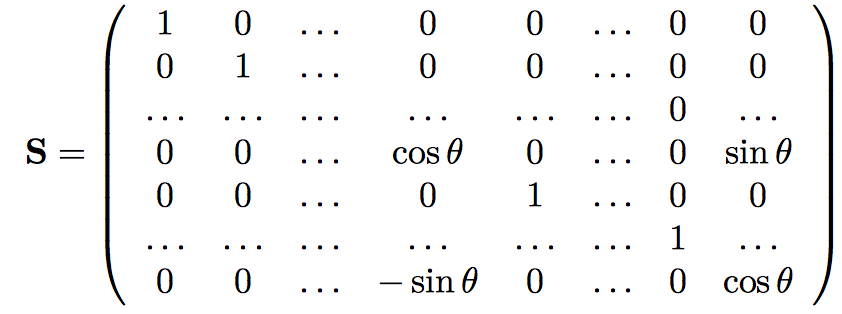
\includegraphics[width=\linewidth]{pict_1.png}
\end{figure}

S performs a plane rotation around an angle $\theta$ in the Euclidean n-dimensional space.
\newline

This means that the matrix elements that differ from zero are given by:
\begin{figure}[h!]

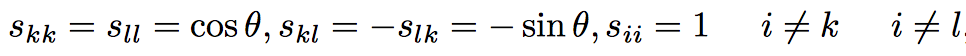
\includegraphics[width=\linewidth]{pict_2.png}
\end{figure}

and the similarity transformation $B = S^T AS$ results in:
\begin{figure}[h!]
  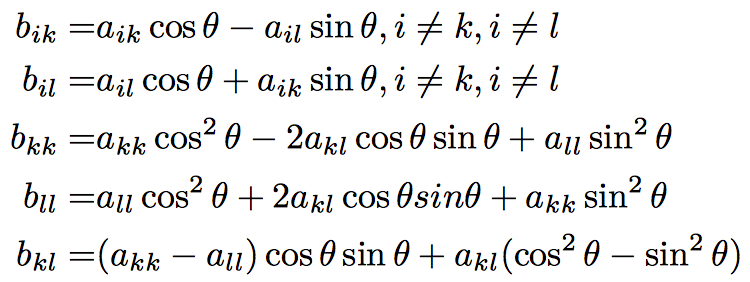
\includegraphics[width=\linewidth]{pict_3.png}
\end{figure}

and here the strategy is to choose $\theta$ so that all the non-diagonal matrix elements $b_{kl}$ become zero. This is what we will code.
\subsection*{Interacting case}
We will also test the same potential but with two interacting electrons in the well. The Schroedinger equation then reads:
\begingroup\makeatletter\def\f@size{8}\check@mathfonts
\def\maketag@@@#1{\hbox{\m@th\large\normalfont#1}}%
\begin{equation*}
\left(  -\frac{\hbar^2}{2 m} \frac{d^2}{dr_1^2} -\frac{\hbar^2}{2 m} \frac{d^2}{dr_2^2}+ \frac{1}{2}k r_1^2+ \frac{1}{2}k r_2^2\right)u(r_1,r_2)  = E^{(2)} u(r_1,r_2) .
\end{equation*}\endgroup
The subscripts indicate each electron in the well with two energies $E^{(2)} = E_{r1} + E_{r2}$. 
We add the coulomb potential because the electrons are now interacting with each other. The coulomb potential states:
\begin{equation*}
V(r_1,r_2) = \frac{\beta e^2}{|\mathbf{r}_1-\mathbf{r}_2|}=\frac{\beta e^2}{r},
\end{equation*}
with $\beta e^2=1.44$ eVnm.
We introduce the relative coordinate r = r1 − r2 and the center-of-mass
coordinate R = 1/2(r1+r2). With these new coordinates, the radial Schroedinger
equation reads:
\begin{equation*}
\left(  -\frac{\hbar^2}{m} \frac{d^2}{dr^2}+ \frac{1}{4}k r^2+\frac{\beta e^2}{r}\right)\psi(r)  = E_r \psi(r).
\end{equation*}
We now do the same manipulation as for the single electron case, introducing a dimensionless variable and simplifying the equation as in eq(5). Ending up with:
\begin{equation*}
  -\frac{d^2}{d\rho^2} \psi(\rho) + (\omega_r^2\rho^2 +\frac{1}{\rho})\psi(\rho) = \lambda \psi(\rho).
\end{equation*}
$\omega_r$ is the strength of the harmonic potential and the potential is now $V(\rho) = \omega_r^2\rho^2 + \frac{1}{\rho}$ which will be tested as well. 
\subsection*{Test functions}
To see if the program is functioning as it should we implement two test functions. The first function tests the jacobi method on a identity matrix and checks if it returns the eigenvalue which is equal to 1 for a small tolerance. The second test examines a input matrix (identity matrix in this case as well) for the maxoffdiag function in program to see if it returns the largest off diagonal matrix element. 
Because of the many lines of code it is favorable to implement test function that checks to see if the code is running properly.
\section*{\Romannum{3}. RESULTS} 
Here we compare the first three eigenvalues for the single electron case using Jacobi and armadillo. The harmonic oscillator potential $V(\rho) = \rho^2$. Eigenvalues are $\lambda_1$ = 3, $\lambda_2$ = 7 and $\lambda_3$ = 11:
\newline
\newpage
\textbf{Table 1: Jacobi vs armadillo}
\newline
\bigskip

\resizebox{3cm} {
\begin{tabular}{|| l | l||}
    \hline
    \lambda_{Jacobi} & \lambda_{armadillo} \\
    \hline 
    2.9995 & 2.9995   \\
    \hline
    6.9975 & 6.9975 \\
    \hline
    10.9939  & 10.9939 \\
    \hline
\end{tabular}
}
\newline
\bigskip

\textbf{Table 1: For n = 200}
\newline
Before checking interacting case we don't include the coulomb potential and see if the eigenvalues with the frequencies coincide with eigenvalues above. We expect that the eigenvalues from table 1 will be multiplied with different $\omega_r$.  
\newline

\textbf{Table 2: Jacobi vs analytic for different frequencies}
\newline
\bigskip
\resizebox{3cm} {
\begin{tabular}{|| l | l | l ||}
    \hline
    $\omega_r$ & $\lambda_{Jacobi}$ & $\lambda_1\cdot \omega_{ri}$\\
    \hline 
    $\omega_{r1}$ = 0.01 & 0.0299 & 0.0299 \\
    \hline
    $\omega_{r2}$ = 0.5 & 1.4874 & 1.4997 \\
    \hline
    $\omega_{r3}$ = 1 & 2.9715 & 2.9995\\
    \hline
    $\omega_{r4}$ = 5 & 14.9214 & 14.9975\\
    \hline
\end{tabular}
}
\bigskip

Now for the interacting case, two electrons in the potential, we compare with analytic solution found for the ground state from [2].
\newline
\bigskip

\textbf{Table 3: Compared eigenvalue with jacobi with analytic}
\newline
\resizebox{3cm} {
\begin{tabular}{|| l | l | l||}
    \hline
    $w_r$ & $\lambda_{Jacobi}$ & Analytic \\
    \hline 
    $w_r$ = 0.25 & 1.24992 & 0.625 \\
    \hline
\end{tabular}
}
\bigskip

\textbf{Table 4: Eigenvalues interacting case}
\newline
\resizebox{3cm} {
\begin{tabular}{|| l | l||}
    \hline
    $w_r$ & $\lambda_{Jacobi}$\\
    \hline 
    $w_r$ = 0.01 &  0.105\\
    \hline
    $w_r$ = 0.5 &  2.2228\\
    \hline
    $w_r$ = 1 &  4.0447\\
    \hline
    $w_r$ = 5 & 17.3664 \\
    \hline
\end{tabular}
}
\bigskip
\newline

Table 4 shows the given eigenvalues with different values of $\omega_r$. 

\subsection*{Link to program}
https://github.com/tobiasolesen/FYS3150-Prosjekt2

\section*{\Romannum{4}. DISCUSSION}
From table 1 the eigenvalues produced from jacobi method match armadillo eigenvalues to the last significant digit. This indicates that the jacobi method is a reliable method for finding eigenvalues also when comparing with analytic eigenvalues $\lambda_1 = 3$, $\lambda_2 = 7$, $\lambda_3 =11$. 
Adding the frequency $\omega_r$ expected values were prodcued from table 2. The number of mesh points needed for getting eigenvalues to 4 leading digits was found to be 200 with 66618 similarity transforms to get off diagonal elements equal to zero.


As for the two electron case from table 3 the two ground state eigenvalues do not seem to match. This is because of the difference in scaling for both cases. From the article [2] Taut ends up with an energy that is different by a factor 2 compared to ours, this leads to $E_{analytic} = \lambda_{jacobi}/2 = 0.625$ which gives us the same energy in the ground state.

The test functions passed when running the program, but for test function finding the max offdiagonal element wasn't of much use when the matrix we used didn't have any off diagonal elements (identity matrix). Testing the jacobi work fine and was a good test to see if the jacobi method passed. Not a problematic test, but a secure one. 

Changing the strength of the potential gives us larger eigenvalues thus higher energies for the increasing frequencies, which is expected when the potential energy is increased the total energy of the system is increased.   
\section*{\Romannum{5}. CONCLUSION} 
The jacobi method is a method giving us the eigenvalues to a certain eigenvalue problem with high accuracy. It turned out to be necessary to scale the equations (for single and two electrons) so that the form of the equation was simplified thus minimizing errors. It was only needed to change the potential of the Schrodinger equation to exemplify the two electron case after scaling. 

It was also good to test the algorithm to see if it at all worked on a simple matrix to exclude certain errors in the algorithm thus saving some time on the error searching.  
\section*{\Romannum{6}. REFERENCES}
[1] http://physics.gmu.edu/~dmaria/590%20Web%20Page/public_html/qm_topics/hydrogen_atom/hydrogen_atom.htm
\newline
[2] https://journals.aps.org/pra/pdf/10.1103/PhysRevA.48.3561
\newline
[3]Hjort -Jensen Morten., 2015. Computational Physics Kompendiet. 
\newline
http://compphysics.github.io/ComputationalPhysics/doc/pub/linalg/pdf/linalg-print.pdf
\end{document}